\documentclass{beamer}

\usepackage{../cppenv}
\usepackage{../recdefs}

\usetheme{Berlin}
\usecolortheme{beaver}

\title{CS100 Recitation 10}
\author{GKxx}
\date{April 25, 2022}

\AtBeginSubsection{
    \begin{frame}{Contents}
        \tableofcontents[currentsection, currentsubsection]
    \end{frame}
}

\begin{document}

\begin{frame}
    \maketitle
\end{frame}

\begin{frame}{Contents}
    \tableofcontents
\end{frame}

\section{Review}

\begin{frame}{Review: Inheritance}
    Inheritance:
    \begin{itemize}
        \item \textbf{`is-a'} relationship
        \item Every object of subclass type contains an object of the base type. Every member except ctors and dtors is inherited, no matter what access level it is of.
        \item Subclass cannot affect behaviors of operations performed on base objects.
        \pause
        \item Behavior of ctors and dtors?
    \end{itemize}
\end{frame}

\begin{frame}{Review: Dynamic Binding}
    Dynamic binding:
    \begin{itemize}
        \item A reference or pointer to the base class can be bound to an object of the subclass.
        \item When a \virtual function is called \textbf{through the reference or pointer to the base class}, it will call the correct version according to the dynamic type of that object.
        \item Any polymorphic class must have a \virtual dtor. Why?
    \end{itemize}
\end{frame}

\begin{frame}{Review: Abstract Class}
    Pure virtual functions and abstract classes:
    \begin{itemize}
        \item Definition of pure \virtual functions.
        \item A class with at least one pure \virtual function is an \textbf{abstract class}.
        \item Abstract classes cannot be instantiated. Pure virtual function without definition cannot be called.
        \item The subclass is still abstract if one of the pure \virtual functions in its base class is not overridden.
        \pause
        \item \textbf{Inheritance of interface} vs \textbf{inheritance of implementation}
    \end{itemize}
\end{frame}

\section{Copy Control}

\subsection{Copy and Swap}

\begin{frame}[fragile]{Swap of Vector}
    The \ttt{std::swap} (defined in \ttt{<algorithm>}):
    \begin{cpp}
template <typename T>
inline void swap(T &lhs, T &rhs) {
  T tmp = lhs;
  lhs = rhs;
  rhs = tmp;
}
    \end{cpp}
    \begin{itemize}
        \item Swap is done by three copies.
        \item Inefficient on some special objects, like \ttt{Vector}.
    \end{itemize}
\end{frame}

\begin{frame}[fragile]{Swap of Vector}
    \textbf{Specialize} the template function \ttt{std::swap}.
    \begin{itemize}
        \item Non-template \(>\) template-specialization \(>\) template.
    \end{itemize}
    \begin{cpp}
namespace std {
template <>
inline void swap<Vector>(Vector &lhs, Vector &rhs) {
  // What should we do here?
}
} // namesapce std
    \end{cpp}
    It seems that \ttt{std::swap<Vector>} needs to access the private members.
\end{frame}

\begin{frame}[fragile]{Swap of Vector}
    By convention, we define a public member:
    \begin{cpp}
class Vector {
 public:
  void swap(Vector &other) noexcept {
    using std::swap;
    swap(m_size, other.m_size);
    swap(m_capacity, other.m_capacity);
    swap(m_data, other.m_data);
  }
  // other members
};
    \end{cpp}
\end{frame}

\begin{frame}[fragile]{Swap of Vector}
    Then we can let \ttt{std::swap<Vector>} call that member:
    \begin{cpp}
namespace std {
template <>
inline void swap<Vector>
    (Vector &lhs, Vector &rhs) noexcept {
  lhs.swap(rhs);
}
} // namespace std
    \end{cpp}
    Note that
    \begin{itemize}
        \item we are not adding any more things to \ttt{std}.
        \item in contrast to the default version, our \ttt{swap} functions are \textbf{exception-free}.
    \end{itemize}
\end{frame}

\begin{frame}[fragile]{Copy and Swap}
    Surprisingly, we obtain a copy assignment operator that is both \blue{self-assignment-safe} and \blue{exception-safe}!
    \begin{cpp}
class Vector {
 public:
  Vector &operator=(const Vector &other) {
    auto temp = other;
    swap(temp);
    return *this;
  }
};
    \end{cpp}
\end{frame}

\subsection{Prevent Copying: An Interesting Way}

\begin{frame}{Prevent Copying}
    Make the compiler unable to synthesize the copying oeprations?
    \begin{itemize}
        \item If the class has an uncopyable base class.
        \item If the class has an uncopyable member.
    \end{itemize}
    Which one is better?\\
    \pause
    \blue{Empty Base Optimization (EBO).}
\end{frame}

\begin{frame}[fragile]{Uncopyable Class}
    \begin{cpp}
class Uncopyable {
  Uncopyable(const Uncopyable &);
  Uncopyable &operator=(const Uncopyable &);
};
class Widget : public Uncopyable {
  // We don't define the copy operations.
  // The compiler is unable to synthesize them,
  // because the copy operations of the base class are inaccessible.
};
    \end{cpp}
\end{frame}

\begin{frame}{Private Inheritance}
    Such definition causes problem: A reference or pointer to \ttt{Uncopyable} can be bound to objects of every such class!
    \pause
    \begin{itemize}
        \item \private inheritance: \textbf{The inheritance relationship is a secret.}
        \item Every operation that relies on such relationship cannot be performed, unless in the subclass or \bluett{friend} of the subclass.
        \begin{itemize}
            \item upcasting and downcasting
            \item accessing base members
            \item dynamic binding
            \item ......
        \end{itemize}
    \end{itemize}
\end{frame}

\begin{frame}[fragile]{Private Inheritance}
    \begin{cpp}
class Uncopyable {
  Uncopyable(const Uncopyable &);
  Uncopyable &operator=(const Uncopyable &);
};
class Widget : private Uncopyable {
  // ...
};
    \end{cpp}
    \pause
    \begin{itemize}
        \item This method is outdated from the perspective of C++11, but the way it uses inheritance is inspiring.
    \end{itemize}
\end{frame}

\section{Resource-managing Classes}

\subsection{Surrogate}

\begin{frame}[fragile]{Shape}
    \begin{columns}
        \begin{column}{0.4\linewidth}
            \begin{figure}[h]
                \centering
                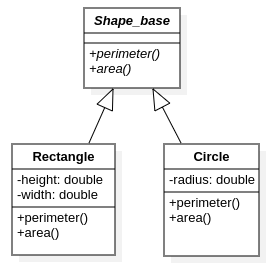
\includegraphics[scale=0.5]{figures/shape_uml.png}
            \end{figure}        
        \end{column}
        \begin{column}{0.7\linewidth}
            \begin{cpp}
class Shape_base {
 public:
  virtual double perimeter() const = 0;
  virtual double area() const = 0;
  virtual ~Shape_base() = default;
  Shape_base() = default;
};
            \end{cpp}
        \end{column}
    \end{columns}
\end{frame}

\begin{frame}[fragile]{Shape}
    \begin{cpp}
class Rectangle : public Shape_base {
  double height, width;
 public:
  Rectangle(double h, double w);
  virtual double perimeter() const override;
  virtual double area() const override;
};
class Circle : public Shape_base {
  double radius;
 public:
  Circle(double r);
  virtual double perimeter() const override;
  virtual double area() const override;
};
    \end{cpp}
\end{frame}

\begin{frame}{Problem}
    How can we define an array of shapes? (also \bluett{new}ed arrays, containers, ...)
    \begin{itemize}
        \item \ttt{Shape\_base shapes[100];} does not work.
        \begin{itemize}
            \item Abstract base class.
            \item Object slicing.
            \item The sting of coworkers' derision.
        \end{itemize}
        \item \ttt{Shape\_base *shapes[100];} seems to work, but...
        \begin{itemize}
            \item What happens when \ttt{shapes[i] = shapes[j];}?
            \item The burden of memory management is on the user's part.
        \end{itemize}
    \end{itemize}
\end{frame}

\begin{frame}[fragile]{Virtual Copy Function}
    How can we copy an object correctly?\par
    \pause
    \textbf{DO NOT} use downcasting like this!!
    \begin{cpp}
Shape_base *clone(Shape_base const *ptr) {
  if (typeid(*ptr) == typeid(Rectangle))
    return new Rectangle(dynamic_cast<Rectangle &>(*ptr));
  else
    return new Circle(dynamic_cast<Circle &>(*ptr));
}
    \end{cpp}
\end{frame}

\begin{frame}[fragile]{Virtual Copy Function}
    Use a group of virtual functions instead.
    \begin{cpp}
class Shape_base {
 public:
  virtual Shape_base *clone() const = 0;
};
class Rectangle : public Shape_base {
 public:
  virtual Shape_base *clone() const override
    { return new Rectangle(height, width); }
};
class Circle : public Shape_base {
 public:
  virtual Shape_base *clone() const override
    { return new Circle(radius); }
};
    \end{cpp}
\end{frame}

\begin{frame}[fragile]{Covariant Return-type}
    \begin{cpp}
class Shape_base {
 public:
  virtual Shape_base *clone() const = 0;
};
class Rectangle : public Shape_base {
 public:
  virtual Rectangle *clone() const override
    { return new Rectangle(height, width); }
};
class Circle : public Shape_base {
 public:
  virtual Circle *clone() const override
    { return new Circle(radius); }
};
    \end{cpp}
\end{frame}

\begin{frame}[fragile]{Defining a Surrogate}
    Avoid manual memory management, while still keep the dynamic binding properties.
    \begin{cpp}
class Shape {
  Shape_base *bp;
 public:
  Shape_base() : bp(nullptr) {}
  double perimeter() const {
    return bp->perimeter();
  }
  double area() const {
      return bp->area();
  }
};
    \end{cpp}
\end{frame}

\begin{frame}[fragile]{Defining a Surrogate}
    \begin{itemize}
        \item All other classes are \textbf{implementation details}, so all their members should be \private (or \bluett{protected}).
        \item Declare \ttt{Shape} as a \bluett{friend} of \ttt{Shape\_base}.
        \item Provide two interfaces \ttt{make\_rectangle} and \ttt{make\_circle}.
        \item \blue{Resource Aquisition Is Initialization, RAII.}
        \pause
        \item Since we allow default construction (so that we can define an array of \ttt{Shape}), we can provide an interface to tell whether \ttt{bp} is \bluett{nullptr}.
        \begin{cpp}
bool is_null() const { return !bp; }
        \end{cpp}
    \end{itemize}
\end{frame}

\begin{frame}[fragile]{Interfaces}
    \begin{cpp}
class Shape {
  friend Shape make_rectangle(double, double);
  friend Shape make_circle(double);
 private:
  Shape(Shape_base *p) : bp(p) {}
};
inline Shape make_rectangle(double h, double w)
  { return new Rectangle(h, w); }
inline Shape make_circle(double r)
  { return new Circle(r); }
    \end{cpp}
    Make sure your surrogate is not influenced by outsider raw pointers!
\end{frame}

\begin{frame}[fragile]{Copy Control}
    Call the virtual \ttt{clone} function.
    \begin{cpp}
class Shape {
 public:
  Shape(const Shape &other)
    : bp(other.bp ? other.bp->clone() : nullptr) {}
  Shape &operator=(const Shape &other) {
    // Be careful with self-assignment!
    auto p = other.bp ? other.bp->clone() : nullptr;
    delete bp;
    bp = p;
    return *this;
  }
  ~Shape() { delete bp; }
};
    \end{cpp}
\end{frame}

\begin{frame}{Homework Exercise}
    Use the copy-and-swap technique to define an assignment operator.
\end{frame}

\begin{frame}[fragile]{Modification}
    Suppose we have some form of modification:
    \begin{cpp}
class Shape_base {
  virtual void stretch(double) = 0;
};
class Rectangle : public Shape_base {
  virtual void stretch(double m) override {
    height *= m; width *= m;
  }
};
class Circle : public Shape_base {
  virtual void stretch(double m) override {
    radius *= m;
  }
};
    \end{cpp}
\end{frame}

\begin{frame}[fragile]{Modification}
    Bitwise-const vs logical-const.
    \begin{cpp}
class Shape {
 public:
  void stretch(double m) { // Should this be const?
    if (bp)
      bp->stretch(m);
  }
};
    \end{cpp}
\end{frame}

\begin{frame}[fragile]{Use the Surrogate}
    Now we can use the shapes smoothly.
    \begin{cpp}
Shape shapes[SIZE];
for (int i = 0; i < n; ++i) {
  if (some_condition(i))
    shapes[i] = make_rectangle(f(), g());
  else
    shapes[i] = make_circle(h());
}
for (int i = 0; i < n; ++i) {
  std::cout << "perimeter == " << shapes[i].perimeter()
            << ", area == " << shapes[i].area()
            << std::endl;
}
    \end{cpp}
    The annoying pointers suddenly disappear!
\end{frame}

\begin{frame}[fragile]{Use of the Original Design}
    \begin{cpp}
Shape_base *shapes[SIZE];
for (int i = 0; i < n; ++i) {
  if (some_condition(i))
    shapes[i] = new Rectangle(f(), g());
  else
    shapes[i] = new Circle(h());
}
for (int i = 0; i < n; ++i) {
  std::cout << "perimeter == " << shapes[i]->perimeter()
            << ", area == " << shapes[i]->area()
            << std::endl;
}
for (int i = 0; i < n; ++i)
  delete shapes[i];
    \end{cpp}
\end{frame}

\begin{frame}[fragile]{Value Semantics and Reference Semantics}
    What will happen when we copy a surrogate object?
    \begin{cpp}
Shape a = somevalue(), b = somevalue();
a = b;
    \end{cpp}
    \begin{itemize}
        \item Value semantics: The object that \ttt{b} points to is copied. (The object is \textbf{unique}.)
        \item Reference sematics: \ttt{a} and \ttt{b} point to the same object. (The object is \textbf{shared}.)
    \end{itemize}
\end{frame}

\begin{frame}{Value Semantics and Reference Semantics}
    Pros and cons?
    \begin{itemize}
        \item Value semantics: always copy the object. Time- and space-costing.
        \item Reference semantics: avoid copying.
        \begin{itemize}
            \item But if \ttt{b} is destroyed, should we destroy the object that \ttt{b} points to?
        \end{itemize}
    \end{itemize}
    \pause
    We want both!
\end{frame}

\subsection{Reference-counting Handles}

\begin{frame}{Reference-counting}
    We define a new kind of `surrogate', named a \textbf{handle}.
    \begin{itemize}
        \item Allow an object to be shared by many handles, and \textbf{set a counter on it}.
        \item Increase the counter when a new handle is pointing to it.
        \item Decrease the counter when a handle no longer points to it.
        \item \textbf{When the counter is decreased to zero, delete the object!}
        \begin{itemize}
            \item ``\textit{A man is dead when he is forgotten.}''
        \end{itemize}
    \end{itemize}
\end{frame}

\begin{frame}[fragile]{Reference-counting}
    \begin{cpp}
class Shape_base {
  friend class Shape;
  int use{1};
  virtual double perimeter() const = 0;
  virtual double area() const = 0;
 protected:
  virtual ~Shape_base() = default;
  Shape_base() = default;
};
    \end{cpp}
\end{frame}

\begin{frame}[fragile]{A Reference-counting Handle}
    \begin{cpp}
class Shape {
  Shape_base *bp;
 public:
  double perimeter() const {
    return bp->perimeter();
  }
  double area() const {
    return bp->area();
  }
  bool is_null() const { return !bp; }
 private:
  Shape(Shape_base *p) : bp(p) {}
};
    \end{cpp}
\end{frame}

\begin{frame}[fragile]{Copy Control}
    Copy ctor and dtor: (Be careful with null pointers!)
    \begin{cpp}
class Shape {
 public:
  Shape(const Shape &other) : bp(other.bp) {
    if (bp)
      ++bp->use;
  }
  ~Shape() {
    if (bp && !--bp->use)
      delete bp;
  }
};
    \end{cpp}
\end{frame}

\begin{frame}[fragile]{Copy Control}
    Copy-assignment operator: Self-assignment-safe!!!
    \begin{cpp}
class Shape {
 public:
  Shape &operator=(const Shape &other) {
    if (other.bp)
      ++other.bp->use;
    if (bp && !--bp->use)
      delete bp;
    bp = other.bp;
    return *this;
  }
};
    \end{cpp}
\end{frame}

\begin{frame}[fragile]{Copy Control}
    This is \textbf{not} self-assignment-safe:
    \begin{cpp}
Shape &operator=(const Shape &other) {
  if (bp && !--bp->use)
    delete bp;
  bp = other.bp;
  if (other.bp)
    ++other.bp->use;
  return *this;
}
    \end{cpp}
\end{frame}

\begin{frame}[fragile]{Where is Copy?}
    It seems that we don't need the virtual \ttt{clone} functions at all! But...
    \pause
    What if we allow some form of modification?
    \begin{cpp}
class Shape {
 public:
  void stretch(double m) {
    if (bp)
      bp->stretch(m);
  }
};
    \end{cpp}
    \pause
    Suppose \ttt{Shape a = b;}. After modification on \ttt{a}, what if we still want \ttt{b} to hold the original object?
    \begin{cpp}
a.stretch(2);
    \end{cpp}
\end{frame}

\begin{frame}[fragile]{Copy on Write}
    Solution: We don't copy the object \textbf{until modification happens}.
    \begin{itemize}
        \item \textit{Laziness is a virtue!}
    \end{itemize}
    \begin{cpp}
class Shape {
 public:
  void stretch(double m) {
    if (bp) {
      if (bp->use > 1) {
        --bp->use;
        bp = bp->clone();
      }
      bp->stretch(m);
    }
  }
};
    \end{cpp}
\end{frame}

\begin{frame}{Standard Library Support}
    Since C++11, the ideas of \textbf{surrogates} and \textbf{reference-counting handles} are supported in the standard library \ttt{<memory>} as \textbf{smart pointers}.
    \begin{itemize}
        \item \ttt{std::shared\_ptr} is a reference-counting smart pointer.
        \item \ttt{std::unique\_ptr} is a surrogate that keeps unique ownership of an object.
        \item \ttt{std::weak\_ptr} might be used for some special purposes.
    \end{itemize}
\end{frame}

\begin{frame}{Reading Materials}
    \begin{itemize}
        \item The ideas in this slides are from \textit{Ruminations on C++} Chapter 5 - 7. Chapter 8 is related to Problem 3 in HW5. An interesting example is in Chapter 9 - 10.
        \item \textit{Effective C++} Item 15, 17 talks about something else related.
        \item \textit{C++ Primer} Chapter 12 (section 12.1) introduces smart pointers.
        \item To know about how to use smart pointers properly, see \textit{Effective Modern C++} Item 18 - 22.
    \end{itemize}
\end{frame}

\end{document}